\def\layersep{2.5cm}

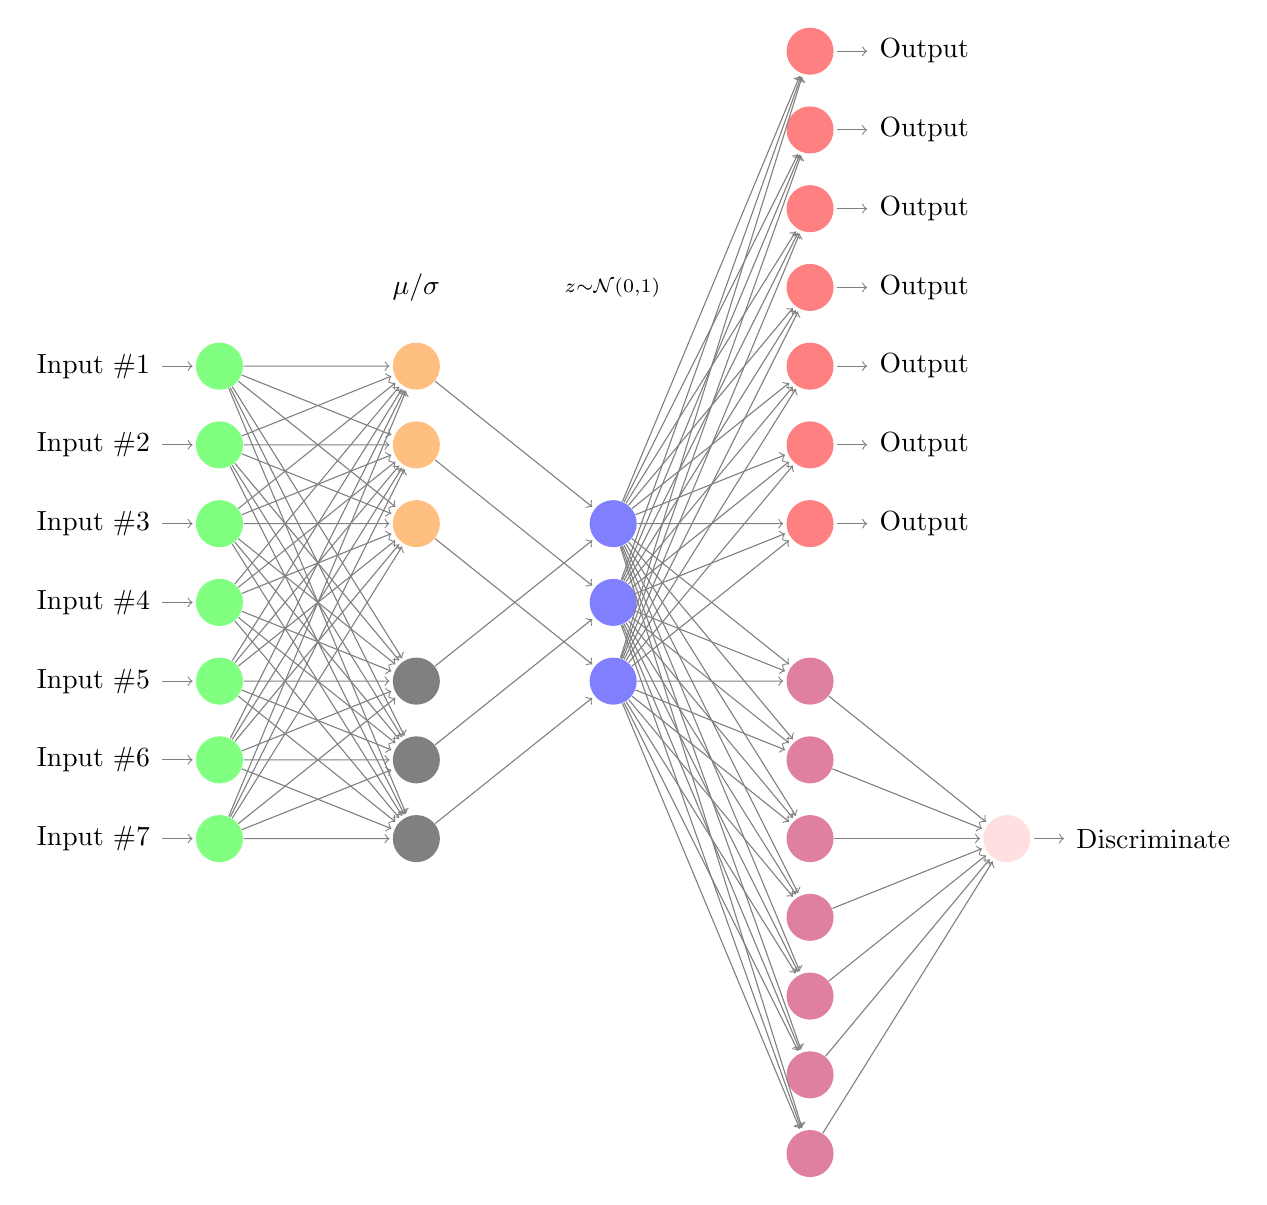
\begin{tikzpicture}[shorten >=1pt,->,draw=black!50, node distance=\layersep]
    \tikzstyle{every pin edge}=[<-,shorten <=1pt]
    \tikzstyle{neuron}=[circle,fill=black!25,minimum size=17pt,inner sep=0pt]
    \tikzstyle{input neuron}=[neuron, fill=green!50];
    \tikzstyle{output neuron}=[neuron, fill=red!50];
    \tikzstyle{discriminator neuron}=[neuron, fill=purple!50];
    \tikzstyle{threshold neuron}=[neuron, fill=pink!50];
    \tikzstyle{hidden mu}=[neuron, fill=orange!50];
    \tikzstyle{hidden sigma}=[neuron, fill=black!50];
    \tikzstyle{hidden neuron}=[neuron, fill=blue!50];
    \tikzstyle{annot} = [text width=4em, text centered]

    % Draw the input layer nodes
    \foreach \name / \y in {1,...,7}
        \node[input neuron, pin=left:Input \#\y] (I-\name) at (0,-\y) {};

    % Draw the hidden layer nodes
    \foreach \name / \y in {1,...,3}
        \path[yshift=-4cm]
            node[hidden mu] (M-\name) at (\layersep, \y cm) {};

    % Draw the hidden layer nodes
    \foreach \name / \y in {1,...,3}
        \path[yshift=-8cm]
            node[hidden sigma] (S-\name) at (\layersep, \y cm) {};

    % Draw the hidden layer nodes
    \foreach \name / \y in {1,...,3}
        \path[yshift=-6cm]
            node[hidden neuron] (H-\name) at (\layersep+\layersep, \y cm) {};

    \foreach \name / \y in {1,...,7}
        \path[yshift=0cm]
            node[output neuron, pin={[pin edge={->}]right:Output}] (O-\name) at (\layersep+\layersep + \layersep,4-\y) {};

    \foreach \name / \y in {1,...,7}
        \path[yshift=0cm]
            node[discriminator neuron] (D-\name) at (\layersep+\layersep+\layersep,-4-\y) {};

    \node[threshold neuron, pin={[pin edge={->}]right:Discriminate}] (T) at (\layersep+\layersep+\layersep+\layersep,-7) {};


    % Connect every node in the input layer with every node in the
    % hidden layer.
    \foreach \source in {1,...,7}
        \foreach \dest in {1,...,3}
            \path (I-\source) edge (M-\dest);

    \foreach \source in {1,...,7}
        \foreach \dest in {1,...,3}
            \path (I-\source) edge (S-\dest);

    \foreach \source in {1,...,3}
        \path (S-\source) edge (H-\source);

    \foreach \source in {1,...,3}
        \path (M-\source) edge (H-\source);

    % Connect every node in the hidden layer with the output layer
    \foreach \source in {1,...,3}
        \foreach \dest in {1,...,7}
            \path (H-\source) edge (O-\dest);

    % Connect every node in the hidden layer with the output layer
    \foreach \source in {1,...,3}
        \foreach \dest in {1,...,7}
            \path (H-\source) edge (D-\dest);

    \foreach \source in {1,...,7}
        \path(D-\source) edge (T);


    % Annotate the layers
    \node[annot,above of=H-1, node distance=5cm] (hl) {${}_{z\sim\mathcal{N}(0, 1)}$};
    \node[annot,left of=hl] {$\mu / \sigma$};
\end{tikzpicture}
